\documentclass{llncs}

\usepackage{times}
\usepackage{graphicx}
\usepackage{url}
\usepackage{verbatim}
%\usepackage{fullpage}

\title{PseudoID: Enhancing Privacy for Federated Login}
\author{Arkajit Dey\inst{1} and Stephen Weis\inst{2}}
\institute{Massachusetts Institute of Technology, Cambridge, MA, USA 02139
\and
Google Inc., Mountain View, CA, USA 94043}

\begin{document}

\maketitle

\begin{abstract}
This paper proposes a privacy-preserving federated login system named
\emph{PseudoID}. PseudoID enhances individual user privacy and
protects identity providers from being compelled to reveal user
data. This system is based on blind digital signatures and is
compatible with a popular federated login system named OpenID. We
propose several extensions and discuss some of the practical
challenges that must be overcome to further protect user privacy.
\end{abstract}

\section{Introduction}
\label{sec:intro}

Internet users often manage login credentials for many accounts across
multiple web sites. This is both an inconvenience and a potential
security risk, as users often resort to reusing passwords. Users also
become accustomed to typing usernames and passwords in many different
interfaces, making them more susceptible to phishing, that is, having
their credentials stolen by spoofed websites.

This has led to several efforts to create web single sign-on (SSO)
systems. One SSO model is for users to have a single \emph{identity
  provider} (IDP) that will be used for all logins. Arbitrary web
sites may then become \emph{relying parties} (RPs), who delegate
logins to the IDP. The IDP handles authenticating the user and
attesting an identity back to the RP.

Some proposals, such as Microsoft Passport (now Windows Live ID)
\cite{MSPass} or Facebook Connect \cite{FBConnect}, relied on a
centralized IDP. Other systems, such as OpenID \cite{OID}, allow users
to have identities from among a federation of IDPs. Federated login
systems like OpenID offer more flexibility to end users, since they
are able to choose among many identity providers. Large webmail
providers like Yahoo, Google, and MSN have all adopted OpenID
\cite{YOP,Sac08,WLOP08} and are capable of serving as identity
providers for hundreds of millions of users.

While federated login systems like OpenID have the prospect of making
logins less cumbersome, they may negatively impact user privacy. The
core problem in both centralized and federated login systems is that
all of a user's logins to relying web sites must flow through their
identity provider. A user's IDP can easily link together the various
websites that the user visits. An abusive IDP could, for example, sell
a list of all the RP's that their users logged into without their
consent.

In a federated system, users could avoid identity providers
that abused privacy and choose to use reputable firms. Unfortunately,
honest identity providers may still be compromised and leak logs, or
otherwise be compelled to reveal logs.

Besides simply revealing which sites a user visits, IDPs often reveal
personal information about users through extensions like OpenID
attribute exchange (AX) \cite{AX} or simple registration (SREG)
\cite{Sreg}. The goal of this exchange is typically to pass
information like an email address, real name, or birthdate from an
identity provider to a web site. Automatically obtaining these data
can greatly streamline the user sign-up process for relying parties.

Although most IDPs will prompt users whether they want to reveal this
information, they could reveal whichever data they want to a relying
party. Thus, there is no way for a user to \emph{selectively disclose}
certain properties (e.g. age, gender, etc.) about themselves to an
RP. Much work has gone into developing cryptographic schemes for
selective disclosure \cite{CaLy01,CaLy04,CHL05,CaGr08}, but these have
yet to be widely adopted in practice.

Finally, the user experience of being redirected back and forth
between the RP and the IDP is less than ideal and especially confusing
to new users. It interferes with the user's well-ingrained mental
model of how they interact with websites.

In this paper, we outline a privacy-preserving federated login system
called PseudoID and offer a sample implementation as an anonymized
OpenID provider. The system utilizes blind signatures \cite{Cha82} and
zero-knowledge proofs \cite{GMR89} to allow users to anonymize
themselves before logging onto RPs. The system exposes a blind
signature service that allows users to generate a digital pseudonym
under which they can logon to a RP, but which cannot be linked back to
their true identity. Additional services are provided to support
selective disclosure of user properties.

\section{Federated Login Overview}
\label{sec:fedlogin}

Web users who want to use a particular website most often authenticate
themselves directly to the site by entering a username and
password. This type of basic web login system has both advantages and
disadvantages. Websites have more flexibility in the design of their
login system, but must carry the burden of authenticating users. These
authentication tasks can be needlessly replicated across many
websites. And, account creation can be a major barrier in signing up new
users. Maintaining many sets of user credentials across different sites also
carries a burden for the user, which can lead to password reuse.
%AD: removed esachs reference for login barrier since I couldn't find a specific
%citation. I feel like it's general enough to not need citation. But if we find
%a good citation later on, we can add it.


%The output of the authentication process is a unique
%identifer such as the username with which the website refers to the
%user in subsequent interactions with him.

\begin{figure}
  \centering
  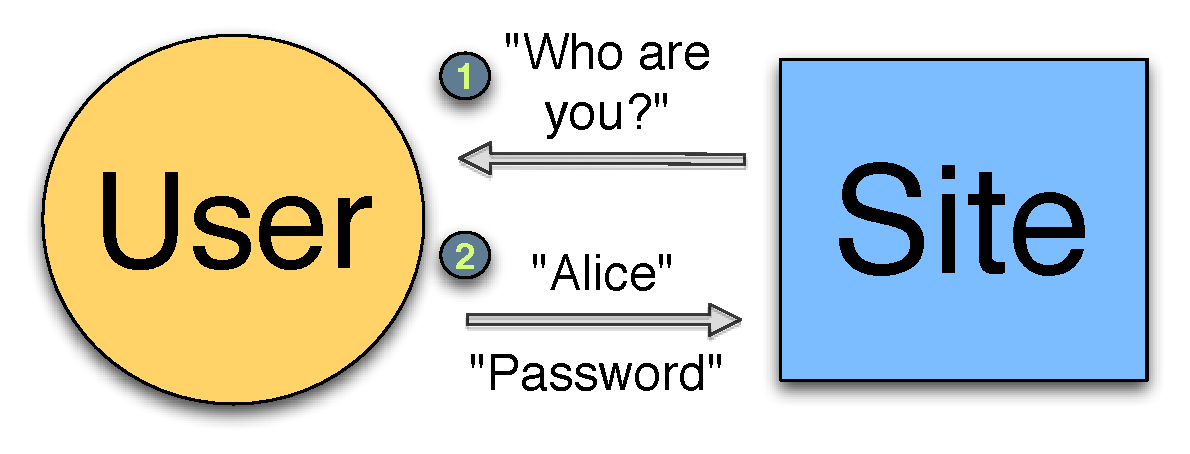
\includegraphics[scale=0.5]{figs/fig-passwd-color.pdf}
  \caption{A familiar web login system where users log into websites
    by entering site-specific credentials.}
  \label{fig:passwd}
\end{figure}

Federated login systems, on the other hand, extract authentication as
a service in its own right. Just as websites rely on third-party services
for traffic analysis, CAPTCHA verification, or file hosting, they can
also rely on separate services for authentication.

Federated login adds a third party to the interaction between the user
and the website: the \emph{identity provider} (IDP). Instead of
authenticating herself to the website directly, the user authenticates
herself to the IDP. The IDP then returns a user identifier to the
website. Thus, the website is often referred to as the \emph{relying
  party} (RP) since it relies on the identity provider for
authentication.

\begin{figure}
  \centering
  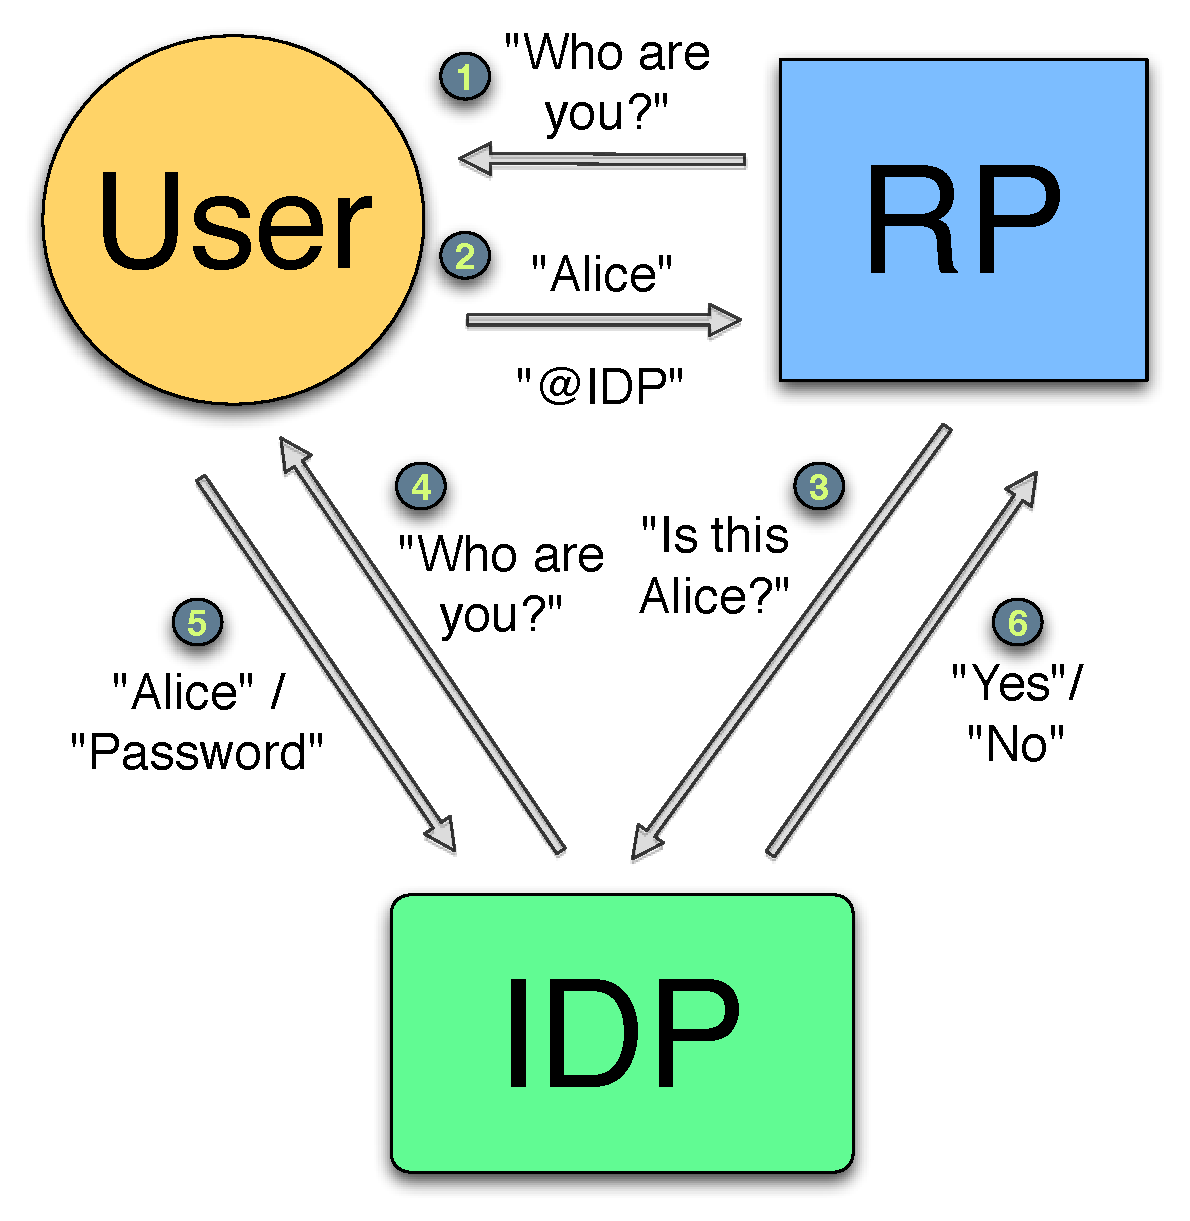
\includegraphics[scale=0.5]{figs/fig-fedlog-color.pdf}
  \caption{A federated login system: the relying party (RP) redirects
  the user to her identity provider (IDP) for authentication.}
  \label{fig:fedlog}
\end{figure}

%The user wishes to use a website which \emph{relies} on the identity
%provider to authenticate the user. Instead of traditional login
%systems where the user authenticates himself to the website directly,
%in federated login systems, the user authenticates himself to the
%identity provider instead. Once the IDP has successfully
%authenticated him, it provides an identity for the user to the RP.
%The RP can then refer to the user through this identifier just as
%they would refer to the user through a username or other handle in
%traditional login systems.

Federated login alleviates the need for websites to store user credentials,
making them less desirable targets for hackers who want to hijack user accounts.
The user benefits from federated login too, as they no longer have to manage
separate login credentials for every website they want to use, and can instead
log into a single IDP. Systems like Facebook Connect and OpenID 2.0 are able to
offer one-click logins for relying parties, which greatly simplifies the login
process. For example, Plaxo, a social networking and address book site,
performed a two-click OpenID login experiment where 92\% of users successfully
completed registration after starting the signup process \cite{Ki09}. (The user
had to click a second time to authorize her identity provider to release her
contact information to Plaxo.)

Accordingly, federated login systems are being adopted by a growing
number of internet sites, particularly by large webmail providers and
social networks.  Several different federated login technologies have
arisen over the years, such as Microsoft Passport (now Windows Live
ID), OpenID, Facebook Connect, and SAML.

%TODO(arkajit): talk more about these systems.

However, popular federated login systems have generally been designed
without privacy as a primary concern. Subsequently, there are risks
with widely-used federated login systems which could put sensitive
user data at risk. The problem of user privacy is indeed magnified in
federated login systems since identity providers act as stewards of
user data for multiple websites. This not only makes them more
appealing targets to attackers, but also more acutely responsible for
safeguarding user privacy.


\subsection{OpenID: A web-based federated login system}

One popular example of a federated login system is OpenID
\cite{OID}. Users can claim identifiers in the form of URIs that will
be attested by their identity provider. To login to a website that
supports OpenID, the user enters their OpenID URI and the RP redirects
them to their identity provider's page. The IDP authenticates the user
through whatever means (e.g. passwords, smart cards, etc.) it desires
and then returns the user to the RP with either a positive or negative
assertion that the user owns the claimed identifier. If the RP
receives a positive assertion from the IDP, it may allow the user to
enter the site under the name of the claimed identifier.

With the advent of OpenID 2.0 \cite{OID2}, the protocol also began to support
the concept of \emph{directed identity} \cite{Cam06} or \emph{private digital
addresses} through a new feature called \emph{identifier select} \cite{RR06}.
This allows the user to just specify the URI of his identity provider instead
of claiming a personal identifier when logging into a website. The site then
redirects the user to the IDP as before, but the IDP now has the opportunity to
select an identifier for the user. Upon successfully authenticating the user,
the IDP returns the selected identifier to the site.

This allows the IDP more flexibility in selecting identifiers for its users. For
example, the IDP may decide to return a different identifier for the same user
for different RPs in order to implement true directed identity as defined in Kim
Cameron's Laws of Identity \cite{Cam06}. And indeed, some OpenID providers like
Google do return a per site unique identifier rather than a globally unique
identifier for its users.

\subsection{Privacy Concerns in Federated Login}

In federated login systems, users entrust identity providers to manage their
identity, so privacy concerns may seem relatively minor. After all, in OpenID
and most other major single sign-on systems, a malicious identity provider could
easily impersonate users to relying parties. However, even if an identity
provider is not corrupt, there are privacy concerns for
\emph{honest, but retentive} providers who may be forced to reveal log data.

The core privacy issue with widely-deployed federated login systems are that
a user's identity can be correlated with the sites they log into. For example,
OpenID identity providers will authenticate users, then redirect them directly
back to a relying party. This makes it trivial to track all the relying parties
a user logs into. This is the same case for Live ID or Facebook Connect; the
identity provider knows all the sites a user logs into.

One might develop a different federated login flow where a user acted as an
intermediary between relying parties and identity providers. The user could
avoid passing any information about the specific relying party to the identity
provider. In this case, the identity provider might return an anonymized
identifier via the user to the relying party. However, if the provider colluded
with the relying party, they could link the user's real identity with the
account on the RP.

An identity provider could abstain from logging, could try to
anonymize or delete identifying information, or could simply destroy
logs completely. Logs are retained for many reasons including
analytics, diagnostics, and security auditing. Abstaining from logging
is generally not a viable option. 

Removing or anonymizing identifying information ex post facto is one
option, but has proved difficult in practice. Supposedly anonymized
logs released by AOL \cite{BarZel06} and Netflix \cite{NaSh08} were
both de-anonymized to some extent. An identity provider would need to
be vigilant and thoroughly scrub logs. They would also need to ensure
that identifying data was not being logged by an unrelated service. 

An added issue is that both logs anonymization and destruction 
may be subject to data retention laws that specify minimum retention
periods \cite{EUDir}. IDPs may be legally compelled to collect
identifying data and retain it for a minimum period.

Given these considerations, we will focus on privacy in a setting where:
(1) identity providers are unable to assure that logs are not retained, and
(2) identity providers may be compelled to reveal logs at some time.

There are several real-world risks where \emph{honest, but retentive}
identity providers may threaten user privacy. One risk is simply if
the provider were compromised and logs were leaked by an
attacker. Another risk is for providers operating in jurisdictions
where logs may be seized without due legal process. 

Because of these risks, identity providers may have an interest in \emph{not}
being able to link a particular user's identity to logins on a particular
relying party. An identity provider may want to provably show that
they cannot link logins on a relying party to a particular user. With
this in mind, we informally define what it means for an idenity
provider to be \emph{private} in Section
\ref{sec:private-fed-login}. Section \ref{sec:pseudoid} propose a
practical system that meets this definition.

\section{Properties of Private Federated Login}
\label{sec:private-fed-login}

For the scope of this paper, we are going to focus on privacy in
federated login systems with an OpenID-like login flow illustrated in
Figure \ref{fig:fedlog}. The relevancy to other types of federated
login systems may vary. 

We assume that identity providers have a set of users that can be
thought of as ``real'' identities. Users may possess credentials which
are presented to identity providers for authentication. If credentials
are valid, identity providers will return some identifier to a relying
party. This identifier may be of any form, i.e. a ``real'' username, a
pseudonym, a value derived from the credentials, or even a random value.

In order to contrast these different behaviors, we will first state
several informal properties.

\begin{definition}[One-wayness]
\label{def:ownership}
An identity provider is one-way if given a specific identifier,
attackers have no significant ability to cause identity providers to
return that value.
\end{definition}

One-wayness means that users actually ``own'' their identities and
people cannot imitate them on relying parties. A trivial example of an
identity provider that is \textit{not} one-way is one where an IDP
will assert any identity without authorizing the user.  We'll refer to
this as the ``Yes IDP''. Users of a Yes IDP could log into RPs with
arbitrary identities, but would not be able to prevent other people
from using the same identities.

\begin{definition}[Consistency]
\label{def:consistency}
An identity provider is consistent if users may present credentials
that will return the same identifier over multiple sessions.
\end{definition}

The consistency property means that users can have long-lived
identities on relying parties. That is, users can log in as the same
identity to a relying party any number of times. A trivial
inconsistent IDP would be one which returned a random value for each
login, or a ``Random IDP''. Users of a Random IDP would be anonymous
on relying parties and could not be linked to their real identities,
but would not be able to establish long-lived accounts on RPs.

\begin{definition}[Unlinkability]
\label{def:unlinkability}
An identity provider is unlinkable if given a transcript of an
authentication event and a set of users, an attacker has no
significant advantage in distinguishing the user being authenticated.
\end{definition}

Unlinkability is intended to capture the notion that an attacker who
obtains access logs from an identity provider and relying party should
not be able to tell which the ``real'' user was logging in.

In practice, OpenID identity providers are generally linkable. An
attacker obtaining a user's credentials or IDP access logs would be
able to trivially see which user was associated with a particular
identity on a relying party.

Note that this property is not specific to OpenID or a flaw in the
OpenID protocol. Instead, it's an artifact of how real world identity
providers typically authenticate users: with usernames and
passwords. An attacker seeing a login event by ``Alice'' followed by
the identity ``Bob'' being returned to a relying party now knows who
``Bob'' is on that RP.

Thus, an unlinkable relying party must not require any identifying
information about their real users during the federated login
protocol. The Yes and Random IDPs mentioned before are in fact
unlinkable, but are not practical in many use cases since they are
respectively not one-way or consistent.

A practical unlinkable system must be both one-way and consistent, and
preferably should have an interactive setup. We now will present such
a system in Section \ref{sec:pseudoid}.

%In addition to preventing tracking by the identity provider, there are several
%other qualities that a privacy-preserving federated login system should
%have. The system should still allow the user to login consistently under her
%selected alias. That is, subsequent visits to a website by a user whose nickname
%is ``Alice'' should be able to be correlated. Further, the system should permit
%the user to control how her nicknames are linked across various relying parties.
%For example, she should be able to decide whether her identity on her bank site
%and her hospital site should be the same (linkable) or different (unlinkable).

%While maintaining these properties, the system should also minimize its trusted
%components, be reasonably resillient against spammers, and be applicable to any
%type of federated login system.

%A \emph{private federated login} system should try to satisfy the following
%goals:

%\begin{enumerate}
%  \item \textbf{Consistent Login}: A user should be able to correlate multiple
%  visits to a website with the same alias.
%  \item \textbf{User-Controlled Linkability}: The user alone, and not her IDP or
%  any RPs, should be able to decide whether any two of her aliases on separate
%  RPs should be linked together.
%  \item \textbf{Minimal Trust}: The system should minimize its trusted
%  components. That is, even a malicious IDP or a set of colluding RPs, should
%  not be able to violate the system's guarantees for the user's privacy.
%  \item \textbf{Cheater Resillient}: The system should incorporate some
%  protections against abusive users such as spammers.
%  \item \textbf{Usability}: The system should be as easy to use as possible and
%  try to prevent the user from making any catastrophic errors such as
%  inadvertently revealing her identity.
%\end{enumerate}

%TODO(arkajit): add a point about selective disclosure here? need to flesh that
%out a bit more...

% \subsection{The ``Yes'' Identity Provider}

% The simplest identity provider is the one who simply authenticates any user who
% asks with a random identifer. While this is ideal for one-time anonymous logins
% to websites, it is really impractical for most users since it fails to offer
% them a consistent identity with which to login. And relying parties suffer as
% well since they accumulate many one-time use accounts that they cannot correlate
% which severely limits their ability to provide a useful service to the user.
% Needless to say, users cannot link identities across multiple websites either.
% Further, such a system imposes no restrictions on would-be spammers and thus
% violates our fourth criterion too.

% \subsection{The Random Identity Provider}

% A slight improvement on the ``Yes'' identity provider is the random IDP which
% does the following. The first time a user visits, it tags them with a random
% identifier and returns it to the relying party. On subsequent visits, the user
% presents his assigned identifier and the identity provider asserts its
% authenticity to the website.

% This does allow the user to create a consistent persona across multiple RPs, but
% also allows the various RPs to collude to piece together the user's browsing
% history. The IDP, meanwhile, ceases to provide any true service as the user is
% allowed to generate his own arbitrary nicknames to login. In particular, there
% are no protections against two users picking the same nickname and effectively
% sharing an account on the RP.

% \subsection{No Identity Provider}

% Finally, the degenerate case is where there is no identity provider at all, i.e.
% the user resorts to the simple traditional per-site login. This is the status
% quo, where the user creates different nicknames (usernames or handles) at each
% website and must remember passwords manually or through a password manager. If
% the user wants to link his identities on two websites, he may decide to choose
% the same nickname on both. But since each site has its own namespace of
% usernames, there is no guarantee that the user ``Alice'' on one site is the same
% as the user ``Alice'' on another site. Moreover, this presents a terrible user
% experience as the user is prone to making privacy-compromising errors. Overall,
% such a setup is not a system at all, is very brittle, and not extensible towards
% new features such as selective disclosure of user attributes to relying parties.

\section{PseudoID: A privacy-preserving federated login system}
\label{sec:pseudoid}
%TODO(arkajit): eliminate abbreviations in prose, OK for diagrams

%a blind signature service (BSS) or blind
%signer, an attribute authentication service (AAS), and a private identity
%provider (IDP). The login flow with PseudoID consists of a one-time setup %phase and then a simplified sign-on phase whenever the user needs to %authenticate to her
%identity provider.

%This access token then allows the user to login to the identity provider
%pseudonymously under their chosen nickname. The system requires that the
%identity provider trust the blind signer to authenticate users on its behalf.
%The identity provider in turn offers authentication services for other relying
%parties that the user wishes to use.

%In practice, the blind signer and the identity provider may even be the same
%entity or at least closely linked (e.g. bss.google.com and idp.google.com).

PseudoID is designed to be a one-way, consistent, and unlinkable federated login system. It consists of a token service used during setup, and a private identity provider used for sign-ons. The user has an account with the token service, which may be a persistent, ``real'' identity like an email address. During setup, the user logs on to the token service using a familiar authentication scheme, such as entering a username and password.

The user then requests an access token from the token service that is bound to a desired pseudonym. When logging into a relying party, the user presents this token to an identity provider. The identity provider will verify the authenticity of the token and return the user's pseudonym to the relying party.

To be unlinkable, the access tokens must be generated such that even if both the token service and identity provider are compromised, the user's ``real'' identity with the token service cannot be linked to their pseudonyms on different relying parties. PseudoID achieves this property by employing \textit{blind signatures}.

\subsection{Blind Signatures}
\label{section:blind-sigs}

Traditional public key digital signature schemes \cite{DH76} consist of a
private signing function $\sigma$ known only to the signer and a public verifying predicate $V$. Then for any message $m$ that is provided to the signer to be signed, a verifier can check that $V(m, \sigma(m))$ is true.

Blind signature systems \cite{Cha82} augment this traditional scheme with a
blinding function $B$ and its inverse unblinding function $B^{-1}$, such that
$B^{-1}(\sigma(B(m)) = \sigma(m)$ and both functions are known only to the
provider.

The provider wishes to obtain a signature $\sigma(m)$ on some message $m$ without revealing the contents of $m$ to the signer. Thus, the provider sends the blinded message, $B(m)$, to the signer. The blinded message leaks no information about $m$ to the signer. The signer then signs the blinded message and returns $\sigma(B(m))$ to the provider. Finally, the provider unblinds this signed message to obtain $$B^{-1}(\sigma(B(m))) = \sigma(m),$$
a valid signature on $m$ that can be publicly verified.

One example of a blind signature system is Chaum's RSA blind signatures. In a
standard RSA digital signature system, the public parameters are a modulus $n$
and an exponent $e$. Only the signer knows the private exponent $d$.

To blind a message $m$ prior to sending it to the signer, the provider multiplies it by a random blinding factor $r$ to produce $B(m) = mr^e$. The signer signs $B(m)$ to produce $$m^d r^{ed} \equiv m^d r \pmod n$$ by Euler's theorem. Since the provider can compute $r^{-1}$, he can unblind the returned signature to obtain $$m^d \pmod n,$$ a valid signature on the original message $m$.

%TODO(arkajit): cite more blind sig scheme examples like El Gamal

\subsection{Blind Token Service}

PseudoID employs a blind signing service (BSS) or \textit{blind signer} that generates blinded access tokens. These tokens are redeemed with an identity provider and used to derive identifiers that are returned to relying parties. This setup phase is outlined in Figure \ref{fig:bss-setup}.

During a setup phase, the user will visit the blind signer and login to an existing account. The user then selects a pseudonym that they want to use on a relying party. This pseudonym is bundled into an access token that the blind signer will sign.

To prevent the signer from being able to link a user with her pseudonym, the user first blinds the token before sending it to the blind signer. The blind signer will sign this token without and return it to the user. Upon receiving the singed token back from the service, the user unblinds it to obtain a signed token that contains the user's chosen pseudonym. Note that the blind signer will not see the user's pseudonym in the clear; it will only see the blinded token.

\begin{figure}
  \centering
  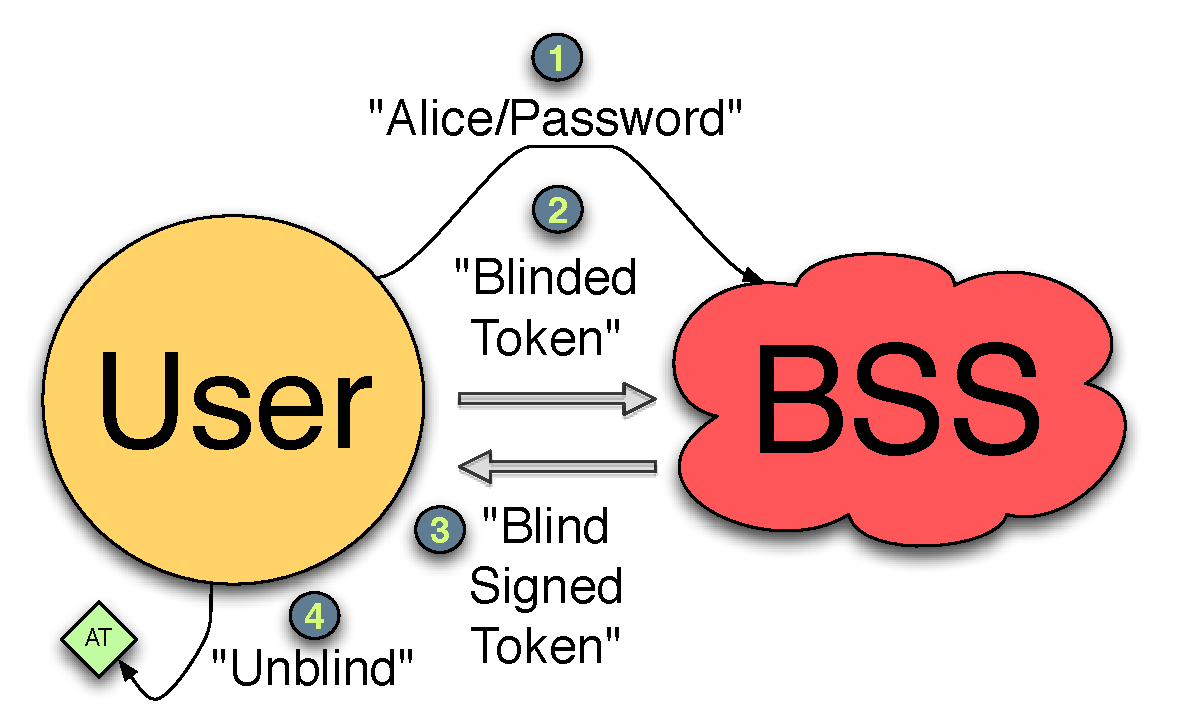
\includegraphics[scale=0.6]{figs/fig-bss-setup-color.pdf}
  \caption{Blind Signer Setup: (1) User first authenticates herself to the BSS
  normally. (2) Then the user sends the BSS a blind token to sign. (3) The BSS
  signs the token and returns it. (4) The user unblinds the blind signed token
  to obtain a valid, untraceable access token (AT).}
  \label{fig:bss-setup}
\end{figure}

\subsection{Private Identity Provider}

The identity provider relies on the blindly signed tokens to be able to authenticate users without forcing them to reveal their identity. When a user is redirected to her identity provider by a relying party, the provider checks whether the user has an access token that has been signed by the blind signer.

The signature on the token may be either publicly verifiable or privately verifiable. In the former case, the identity provider can verify the signature on the access token using the blind signer's public key. In the latter case, the identity provider could send the token to the blind signer and ask them whether they signed it. The sign-on process using an access token in the publicly verifiable case is illustrated in Figure \ref{fig:bss-signon}.

\begin{figure}
  \centering
  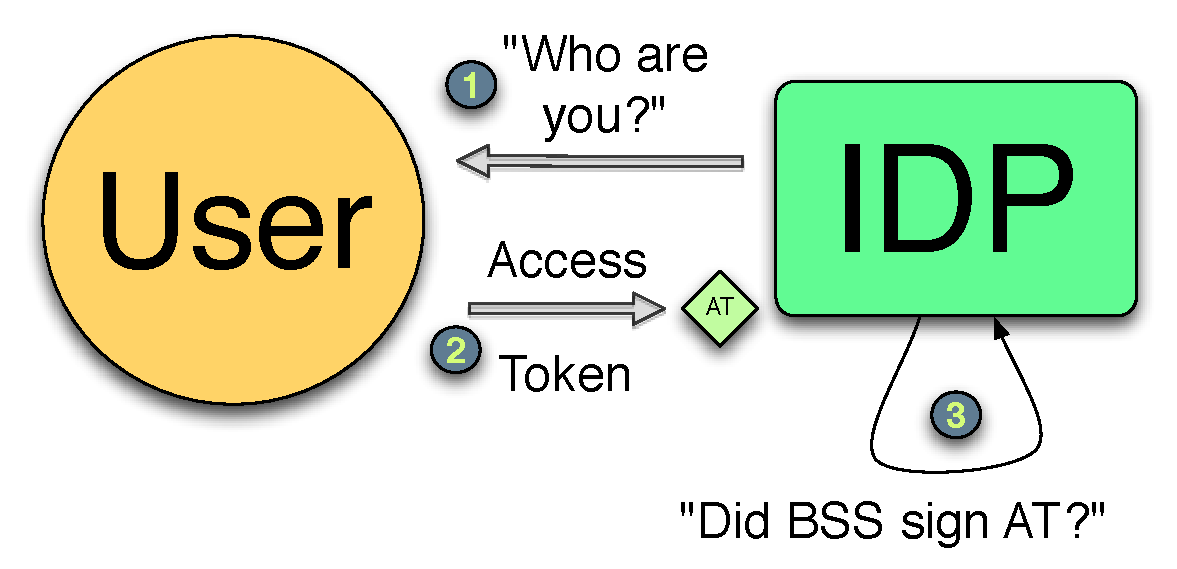
\includegraphics[scale=0.6]{figs/fig-bss-signon-color.pdf}
  \caption{Identity Provider Signon with Blind Signed Access Token: (1) IDP asks
  users to authenticate (2) User supplies access token rather than true identity
  or credentials (3) IDP verifies whether BSS signed the token using BSS's
  public key.}
  \label{fig:bss-signon}
\end{figure}

If the access token is valid, the provider is only assured that the user has been authenticated by the blind signer. Thus the provider knows that the user is a valid user of the blind signer, but does not know which user.

%Deprecated figure, too complex, replaced by two smaller figures
\begin{comment}
\begin{figure}
  \centering
  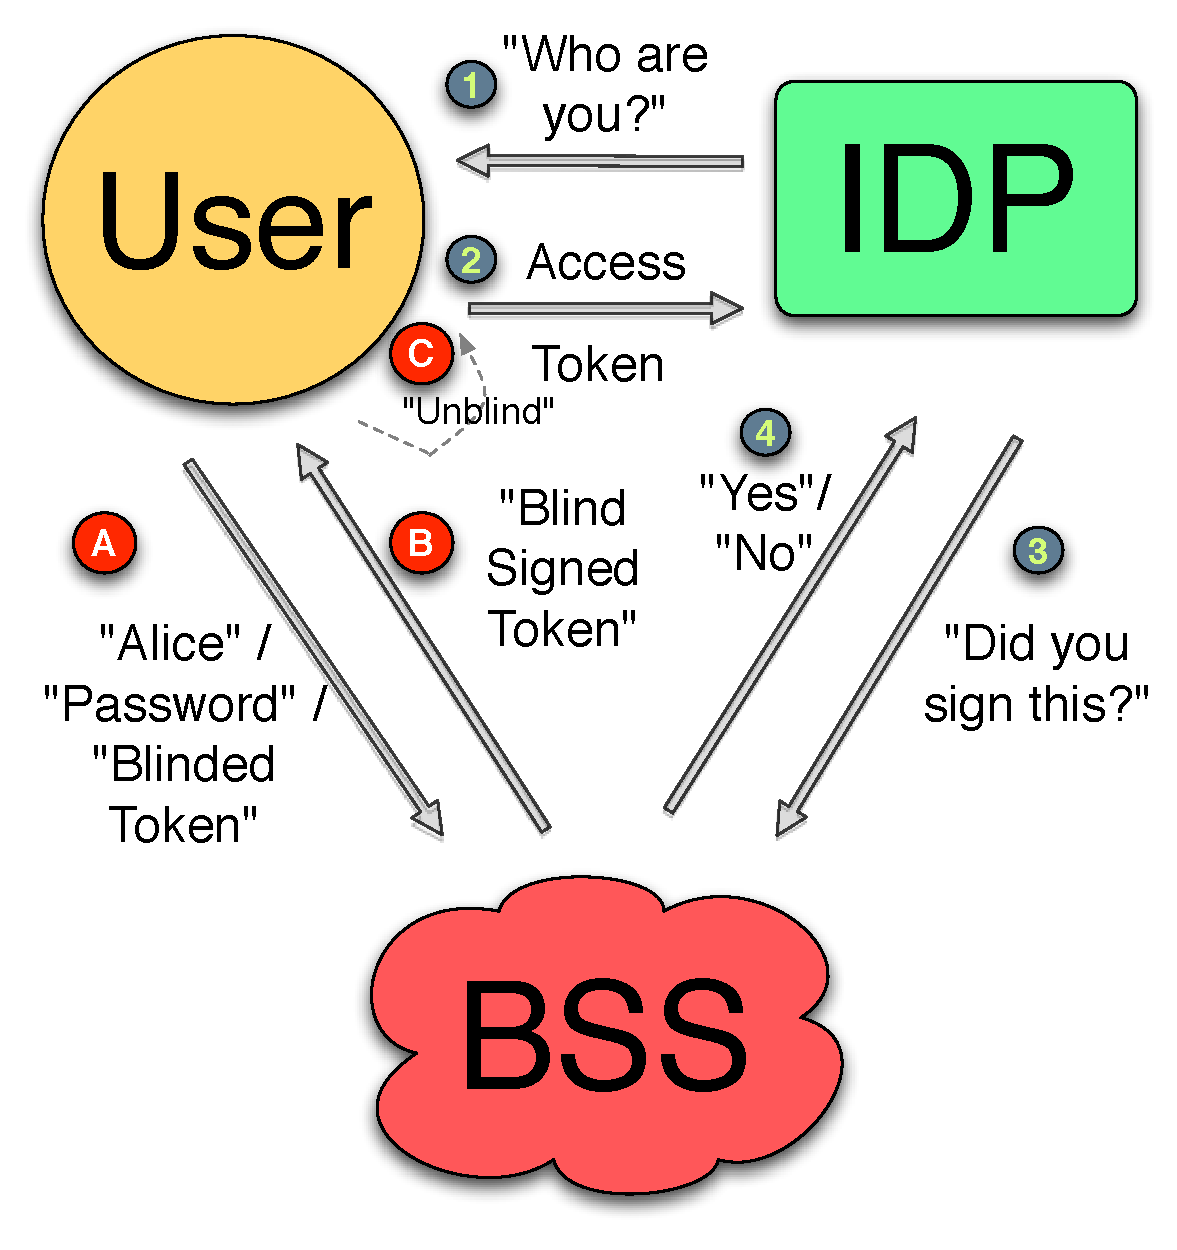
\includegraphics[scale=0.6]{figs/fig-bss-color.pdf}
  \caption{The user obtains an untraceable access token from the blind signature service prior to logging into a website. When his identity provider asks him to authenticate, he provides the access token instead of a username or password. The identity provider, in turn, verifies that the BSS signed the token. If the token has been validly signed, the provider authenticates the user to the website he is trying to visit.}
  \label{fig:bss}
\end{figure}
\end{comment}

%A simple access token may contain just a pseudonym, but may also conThe access token may be imbued with certain semantics such as an embedded
%pseudonym. Upon verying that the access token is legitimate, the identity
%provider may extract the pseudonym from the token and assert its validity to %the
%relying party. Finally, the user is able to login to the website under this
%pseudonym.

\subsection{OpenID with PseudoID}

PseudoID is practical to implement in a web-based model appropriate for OpenID. The blind signer may be implemented as a web service. Users visit the blind signer and can prepare a blinded token to be signed either via a browser plug-in or JavaScript (see Section \ref{subsec:caveats} for a discussion of some caveats of JavaScript). The blind signer will blindly sign this value and return it to the user. This value is unblinded and stored as a cookie in the user's browser. This cookie will be set on the identity provider's domain.

The identity provider itself may be slightly modified from existing OpenID providers. It simply needs to read an access token from a cookie on the user's browser, verify a signature on it, and return the pseudonym it contains to a relying party. From the user's perspective, this eliminates the need to retype a username and password on an identity provider.

PseudoID identity providers are fully compatible with existing OpenID relying parties. Existing relying parties do not have to change anything about their current OpenID flow in order to be able to accept users from private identity providers. From the perspective of the relying party, a private identity provider is indistinguishable from a regular provider. A private provider simply uses a different authentication mechanism than most other identity providers, but it still participates in the same federated login flow outlined in Figure \ref{fig:fedlog}.

\subsection{Caveats}
\label{subsec:caveats}

%System Caveats: Potential for traffic analysis. Need to manage tokens.

%Implementation caveats: Cookies are weak. Need to tunnel through TOR
%and scrub browser. Running crypto in Javascript is unsafe; need to
%trust code.

PseudoID stores a user's access tokens as cookies in the browser. This is not the ideal solution. Many users clear cookies frequently or use a private browsing mode, and thus would lose their blinded access token. Cookies are also set in a single browser, and thus would be difficult to extend a user's pseudonym across different machines.

There is also a security issue with setting a cookie on the identity provider's domain. JavaScript executing on one domain cannot set a cookie on another. The proof-of-concept PseudoID implementation must make a call to the identity provider to set an unblinded cookie during the setup phase. This means that access logs on the blind signer and the identity provider could be joined to correlate the user's login with the value that was set as a cookie.

Even if logins are private, user requests can still be tied to a particular IP address. This method of tracking can be fragile since users may be using proxies or otherwise hidden behind network address translators (NATs) \cite{Pool00}. Even this method may be avoided if the user uses anonymous browsing technology like Tor \cite{Tor}.

In practice, cookies are most often used to track users than IP Addresses. To ensure that the blind signer is not maliciously tagging the user with a uniquely identifying cookie when the user logs into to create their anonymous access token, it may be necessary to scrub all cookies not associated with PseudoID after visiting the blind signer.

Furthermore, the JavaScript code that performs the blinding and unblinding
operations on the BSS must come from a trusted source.

\subsection{Performace and Cost}

Get latency costs using firebug. Blast GAE with requests. How many to
exhaust the quota? Use that to extrapolate the cost of running a blind
signer.

(This might be an uninteresting section.)

\section{Practical Challenges}

There are several practical considerations dealing with implementation issues as
well as usability.

\subsection{Cryptography in the Browser}

Cryptographic computations often rely on number theoretic manipulations of big
integers, i.e. infinite precision integers, not just normal 32-bit integers. We
used the JSBN library to handle big integer computations in Javascript
\cite{Jsbn}.

\subsection{Cross-Domain Communcation}

Another main challenge was communicating cryptographic tokens across domains
subject to the constraints of the \emph{same-origin policy}. It defines two
pages to have the ``same'' domain if they originate from the same protocol,
host, and port. Thus, for example, a page on the blind signer's domain cannot
set a cookie on or make an AJAX call to the private identity provider's domain.

There are many popular techniques for skirting the same-origin policy such as
using fragment identifiers \cite{Adi07}, nested frames \cite{JaWa07}, or cross-
domain scripts to pass messages between domains.

While the same-origin policy prevents unintentional cross-domain communication
between non-cooperative domains, it still permits communications between
cooperative domains. And in PseudoID, the blind signer and the private identity
provider are indeed cooperative entities.

Thus one simple way of exchanging information between the blind signer and the
identity provider is to load a hidden cross-domain iframe. This technique was
used to allow the blind signer to set a cookie on the identity provider's
domain.

When the user generates his access token, he is on the blind signer's domain. By
the same-origin policy, this access token could not be set directly as a cookie
on the identity provider's domain. But the blind signer can source an iframe to
the identity provider and pass a message in the source URL's fragment
identifier. The identity provider can extract the message from the fragment
identifier. Thus the blind signer may send the cookie as a message that the
identity provider may then set on its own domain.

\section{Extensions and Future Work}

Attribute exchange. Using zero-knowledge proofs instead of Chaum's
blind signer to enable more rich and efficient selective
disclosure.

Cookie same origin policy is a hinderence. We want the ability for our
browser to set a value that is only readable by another domain. Need
plug-in or HTML5 feature?

Changing flow of OpenID: User can pass token to RP, they can verify
directly with IDP. Neither RP nor IDP learn the user's actual
identity. Could be more efficient and usable than OpenID (plus lays
groundwork for Ben and Moti's patent.)

Just citing everything to debug the bib file~
\cite{Cha82,Cha85,GMR89,Json,PyOpenId,ProviderApp,Jsbn,JaWa07,Adi07}.

\bibliography{pseudoid}
\bibliographystyle{acm}

\end{document}

% LocalWords:  login OpenID username
